Machine learning algorithms can figure out how to perform tasks by generalizing, where the goal is to generalize beyond the examples of a training set \cite{18}. The programs using the algorithm learn from data and as more data becomes available, more complex problems can be handled. Systems such as web search, spam filters and stock trading uses this approach.
\\[0.5cm]
Many learning algorithms exist and they are all based on combinations of three components \cite{18}; 1) the \textbf{representation} component makes an attempt to discover how to represent the input during training of the algorithm. What kind of information expressed in the data decides what representation algorithm to use; 2) the \textbf{evaluation} component has the objective of distinguishing between the best and the worst output from the representation component and let the next component decide which choice is the best. Basically it attempts to map the output to a specific value so that the next component can analyze it; 3) finally, the \textbf{optimization} component needs to search for the highest scoring output from the evaluation and then deliver it as a result. A greedy search could be an example of such a search (see figure ~\ref{fig:threeComponents}).
\begin{figure}[h!]
\centering
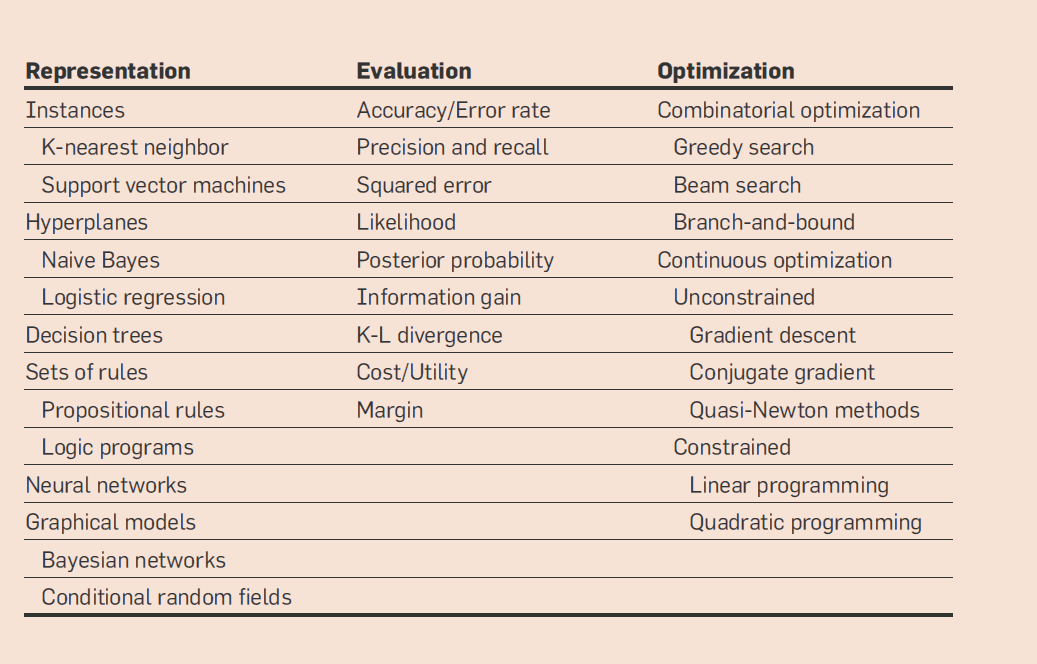
\includegraphics[width=0.6\linewidth,natwidth=898,natheight=587]{billeder/Table1-TheComponentsOfLearningAlgorithms.png}
\caption{The three components of learning algorithms \cite{18}}
\label{fig:threeComponents}
\end{figure}
\\[0.5cm] 
Machine learning cannot rely on data alone. Every learner must make assumptions beyond the data that is given to generalize beyond it \cite{18} because it is not possible to map the real world uniformly to a possible mathematical function. When meteorologists try to model the weather they make assumptions based on historical datasets that are similar to the current weather conditions. If enough historical occurrences resulted in the same weather condition the meteorologists must make the assumption that it can be classified as what have been seen before. The same is applicable when predicting electricity prices. We examine historical data and locate situations that are similar to the current and if enough examples with the same result is found it can be assumed that they are of the same type.
\\[0.5cm]
It can be the case that the system is not at all able to deliver a correct answer. This could result in the system guessing to the best of its ability or simply randoming an answer. This problem is called overfitting \cite{18}. Overfitting can be divided into bias and variance, where bias is when the learner consistently learns the same wrong thing over and over again. Variance is the learner's tendency to learn random things and ignoring the possibility of a more correct answer. See figure ~\ref{fig:biasandvariance} for an example with dart throwing.
\begin{figure}[h!]
\centering
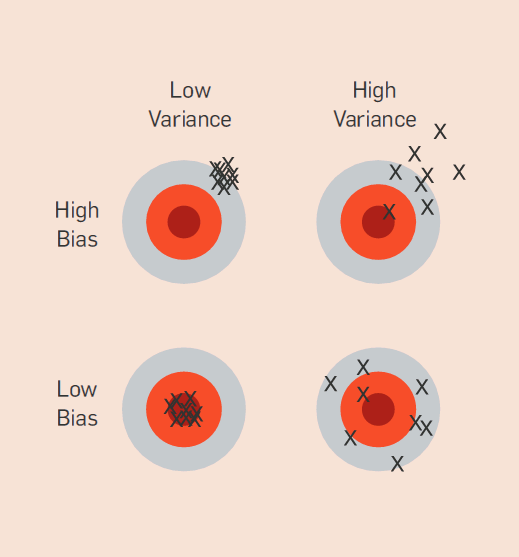
\includegraphics[width=0.5\linewidth,natwidth=898,natheight=587]{billeder/biasVSvariance.png}
\caption{Example of bias and variance in a dart throw \cite{18}}
\label{fig:biasandvariance}
\end{figure}

Machine learning is not only about the technical stuff but it also relies a great deal on intuition, creativity and  black art \cite{18}. 
\newline A way to achieve machine learning is by using a Artificial Neural Network. One way to model an ANN is to base it on the
Levenberg-Marquardt algorithm \cite{7,9,10}. It is a least squares algorithm that,
opposed to Backpropagation algorithm\cite{8}, is very fast at calculating the
results. It is a curve fitting algorithm mostly used on nonlinear problems with
a lot of unknowns[Need citation]. The algorithm can be used with Artificial Neural Networks and information approximation\cite{8} and it can be used in combination with the backpropagation algorithm to be used on a feedforward architecture of the neural network\cite{13}.